\documentclass[12pt]{article}

\usepackage[margin=1in]{geometry}
\usepackage{setspace}
\usepackage{mathptmx}
\usepackage[T1]{fontenc}
\usepackage[utf8]{inputenc}
\usepackage{graphicx}
\usepackage{float}
\usepackage{textcomp}
\usepackage{amsmath}

\doublespacing
\setlength{\parindent}{0pt}
\setlength{\parskip}{0.5em}

\begin{document}

\title{Group Assignment 6: Economic Analysis of Japanese Negative Interest Rates\\[0.5em]}
\author{Logan Rechin, Joe White\\ECO 442}
\date{April 22, 2026}
\maketitle

In March 2024, the Bank of Japan ended its negative interest rate policy and raised interest rates for the first time in seventeen years. In international finance, a higher domestic interest rate should make domestic assets more attractive and lead to an appreciation of the domestic currency therefore strengthening the yen. Instead, the yen weakened after the announcement. This created a very interesting event because it showed that exchange rates respond not just to whether a central bank raises or lowers rates, but to the size of the policy change, the expected future policy, and the gap between domestic and foreign interest rates.

Before analyzing this event, it is important to explain what negative interest rates are and how they are possible. Negative interest rates do not mean that the cash people hold starts losing value on its own. Instead, it means that commercial banks are charged for holding some reserve balances at the central bank. In Japan, the Bank of Japan applied a negative rate to part of the reserves held by financial institutions. The goal was to encourage banks to lend more and to push interest rates lower throughout the economy. Negative interest rates are just an extreme version of expansionary monetary policy. They are possible because the central bank controls the interest rate paid on reserves. As long as banks continue to hold reserves in the system, the central bank can set that return below zero.

There are limitations to negative interest rates. If rates become too negative, banks may become less profitable, and households or firms may prefer to hold cash instead of deposits. This is part of why negative interest rate policy is seen as unusual. Japan used it because the country had struggled for years with low inflation, weak demand, and slow growth. The policy was part of an attempt to stimulate the economy and move inflation closer to the central bank's target.

This should help explain why the March 2024 decision mattered. The Bank of Japan was ending a policy regime that had been associated with Japan's long fight against deflation. Because of that, we expected the yen to strengthen after the announcement. That leads to our economic question: Why Did the Yen Weaken After the Bank of Japan Ended Negative Interest Rates?

To answer this question we should look to the asset market and interest rate parity. Exchange rates are forward-looking asset prices. Investors compare the expected return on domestic deposits with the expected return on foreign deposits. That means the exchange rate depends not only on the current domestic interest rate, but also on foreign interest rates and on expectations about the future exchange rate. A small increase in Japanese interest rates alone would tend to strengthen the yen. However, that effect can be offset if markets still expect foreign assets, especially U.S. dollar assets, to offer higher returns overall.

That is what happened in this case. The Bank of Japan ended negative rates, but rates remained very low even after the increase, while U.S. interest rates were still much higher. As a result, the interest rate differential between the United States and Japan remained large. Markets therefore had little reason to believe that yen assets would suddenly become much more attractive than dollar assets. The symbolic importance of ending negative rates was larger than the actual change in relative returns.

\begin{figure}[H]
\centering
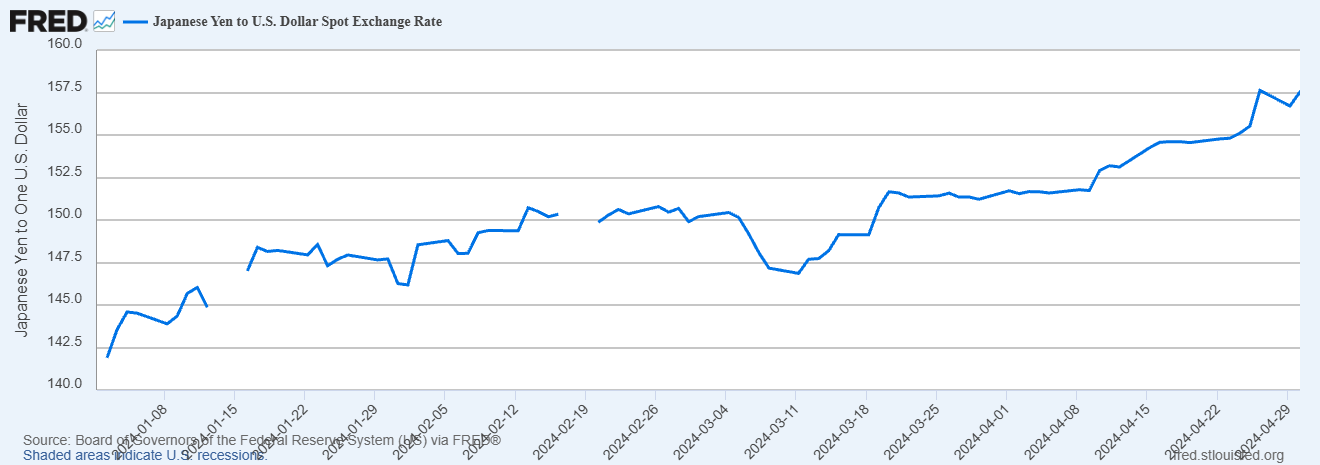
\includegraphics[width=0.82\textwidth]{project_6_graph.png}
\caption{Japanese yen per U.S. dollar March 2024.}
\label{fig:yen_chart}
\end{figure}

Figure \ref{fig:yen_chart} shows what happened to $E_{\text{\textyen}/\$}$ before and after the policy announcement. If financial markets had viewed the Bank of Japan's decision as a strong monetary tightening, we would expect the yen to appreciate after the announcement. Instead, the figure shows that the yen remained weak around the event window.

This shows why the simple statement ``higher interest rates lead to a stronger currency'' is not always true. This can be true if everything else stays the same, but in real financial markets, everything else does not stay the same. What matters is the full policy expectations. If investors believe that Japan will remain cautious while the United States continues to offer higher returns, the yen can still weaken even after a Japanese rate increase. That is exactly what makes this event interesting.

The AA-DD model supports this interpretation. In the short run, prices are sticky, so exchange rate movements are driven mainly by asset markets rather than by immediate changes in goods prices. Tighter monetary policy raises domestic interest rates and causes the currency to appreciate. But the March 2024 decision was not viewed as a major tightening of monetary conditions. Instead, it was seen as a cautious step away from an old policy regime. Since the overall stance of Japanese monetary policy was still soft relative to U.S. policy, the yen did not appreciate how me may have predicted.

Overall, this event is a good example of how international monetary systems function. Negative interest rates were possible because the central bank could set the return on reserves below zero in an effort to stimulate the economy. But ending that policy did not automatically strengthen the yen. Exchange rates depend on expected returns, not just on whether one central bank takes some new stance. What we took from this is that exchange rates are forward-looking, and expectations about future policy can matter just as much as the current change in interest rates.

\begin{thebibliography}{9}

\bibitem{fred_yen}
Board of Governors of the Federal Reserve System (US), \textit{Japanese Yen to U.S. Dollar Spot Exchange Rate} [DEXJPUS], retrieved from FRED, Federal Reserve Bank of St. Louis; \texttt{https://fred.stlouisfed.org/series/DEXJPUS}, April 22, 2026.

\end{thebibliography}

\end{document}